A viscous vortex advection case is performed on a grid, where $\Delta x=\Delta y=\Delta z=0.25$ and $-5\le x \le5$, $-5\le y \le 5$, and $0\le z \le 24$. A vortex profile is fixed at the inlet, where the density and velocity profiles are prescribed according to Eqn.~\ref{vor-equ}, and the pressure is set to be constant at the outlet. Periodic boundary conditions are imposed for the remaining boundaries. The Reynolds number is set to $1.56\times10^6$. The vortex is expected to be dissipated in the stream-wise more severely than the inviscid cases, and the isosurface of vorticity magnitude would resemble a cone.

The test cases are simulated with the baseline MUSCL scheme, the original and the extended eddy-preserving limiter schemes. The unsteady simulations for all schemes start from a converged steady solution computed from the MUSCL scheme. The time step is set to be constant $\Delta t=0.04$, and at final time $t=20$, all simulations have reached quasi-steady states.

The vorticity contours at several stream-wise locations are plotted in Fig. \ref{vortv}. At each location, the EDDY and EDDY-P schemes produce higher vorticity magnitude in the central region than the MUSCL scheme. The isosurface of vorticity magnitude equals one is plotted in Fig. \ref{iso} to show a shape of the vortex. The EDDY and EDDY-P schemes are able to preserve the vortex considerably longer than the MUSCL scheme. The comparisons demonstrate that the EDDY and EDDY-P schemes also outperform the MUSCL scheme for turbulent flow simulations.
%%%%%%%%%%%%%%%%%%%%%%%%%%%%%%%%%%%%%%%%%%%%%%%%%%%%%%%%%%%%%%%%
%%%%%%%%%%%%%%%%%%%%%%%%%%%%%%%%%%%%%%%%%%%%%%%%%%%%%%%%%%%%%%%%
\begin{figure}[t]  
\centering
     \subfigure[MUSCL at $z=1$]{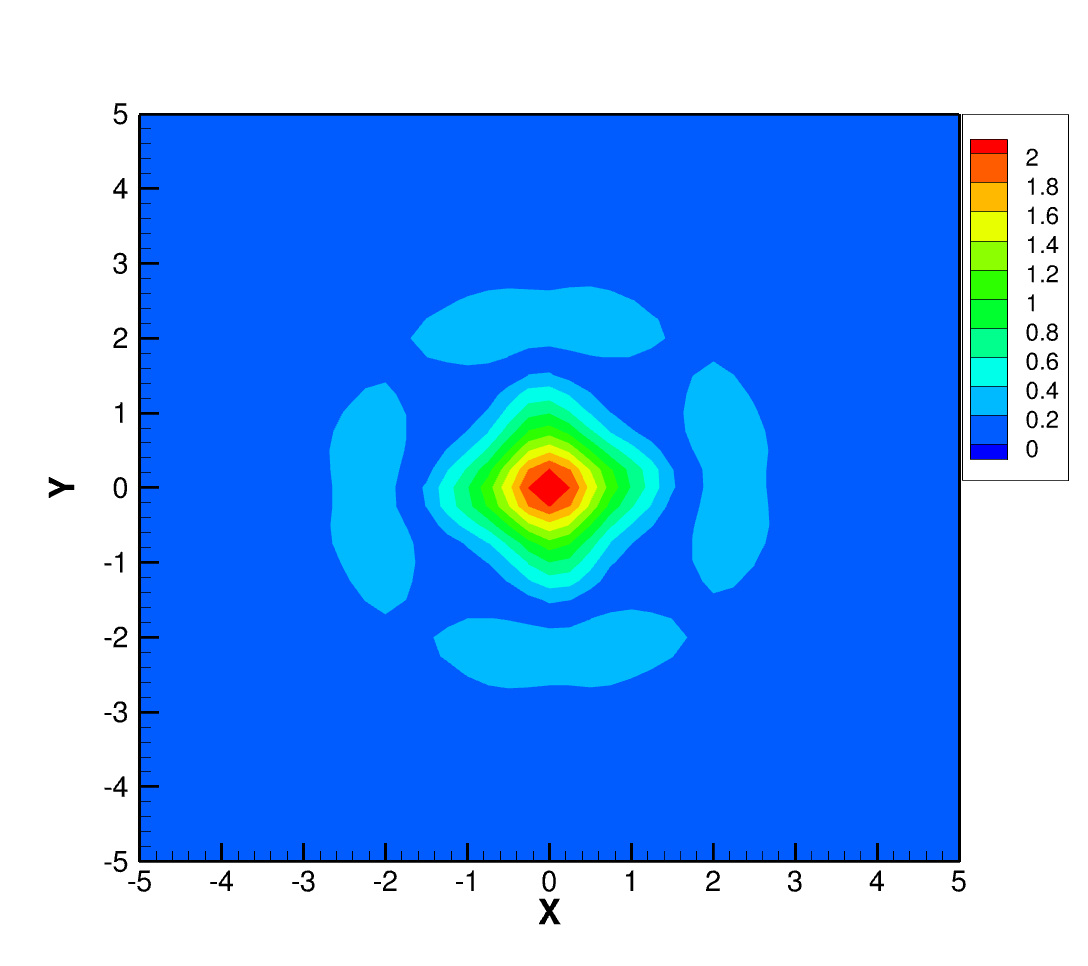
\includegraphics[clip=true, trim= 1.5cm 1.25cm 0.25cm 0.5cm,width=0.325\linewidth]{./figures/vortex3d/viscous/m1}}              
     \subfigure[EDDY at $z=1$]{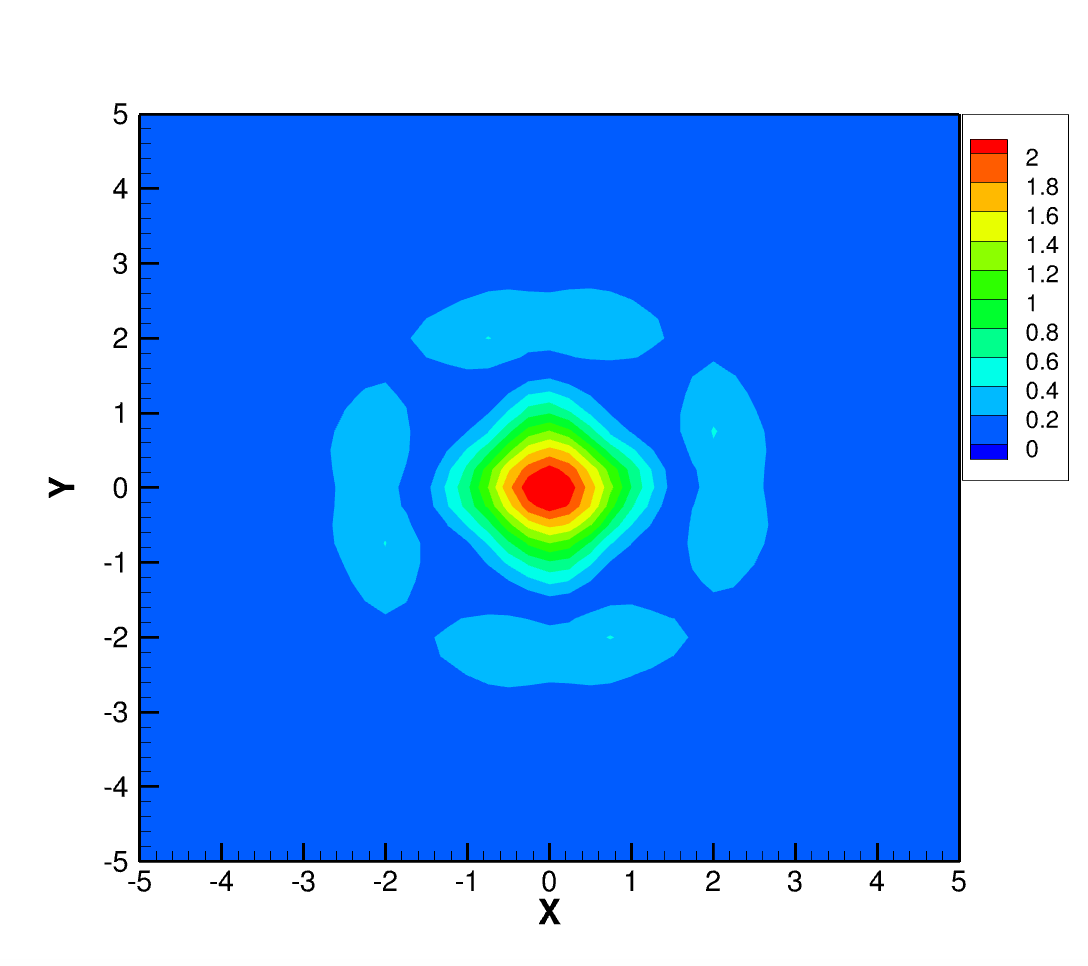
\includegraphics[clip=true, trim= 1.5cm 1.25cm 0.25cm 0.5cm,width=0.325\linewidth]{./figures/vortex3d/viscous/e1}}
     \subfigure[EDDY-P at $z=1$]{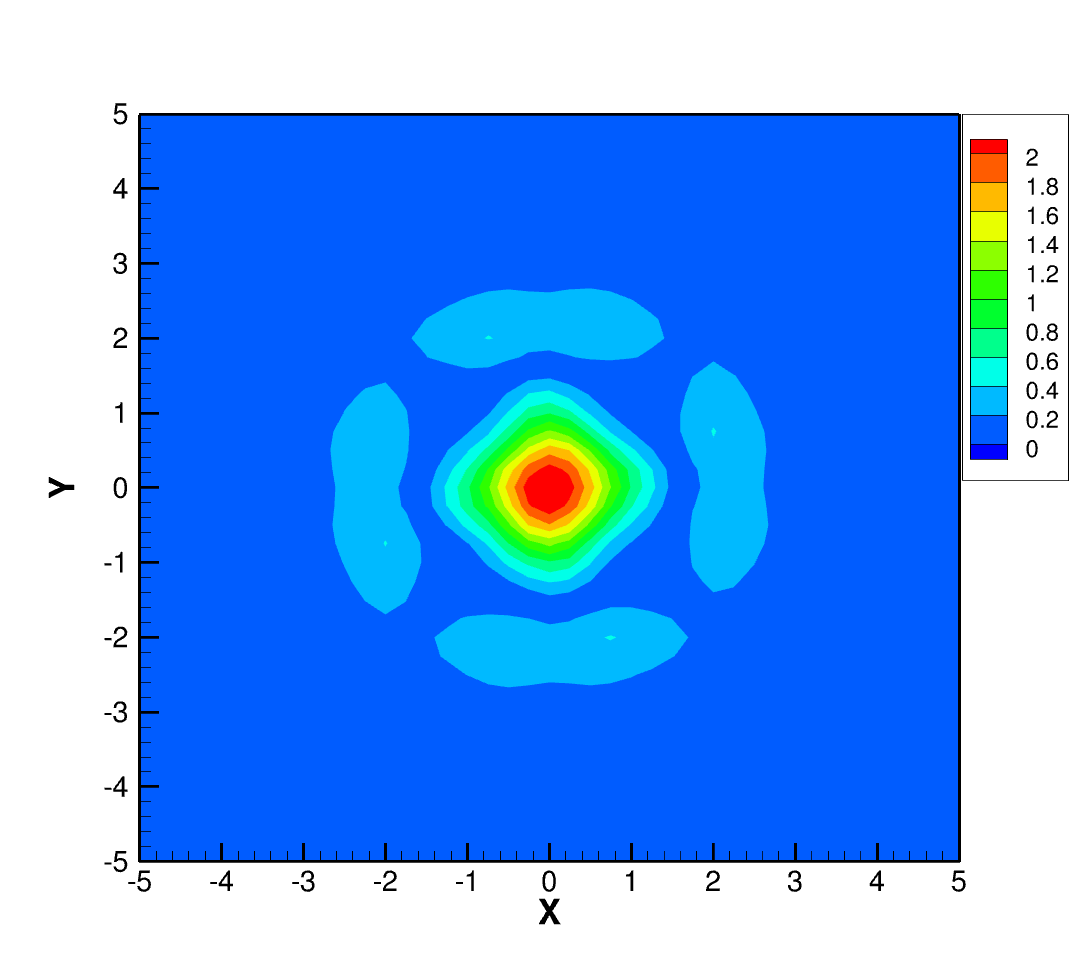
\includegraphics[clip=true, trim= 1.5cm 1.25cm 0.25cm 0.5cm,width=0.325\linewidth]{./figures/vortex3d/viscous/ep1}}
     \subfigure[MUSCL at $z=2$]{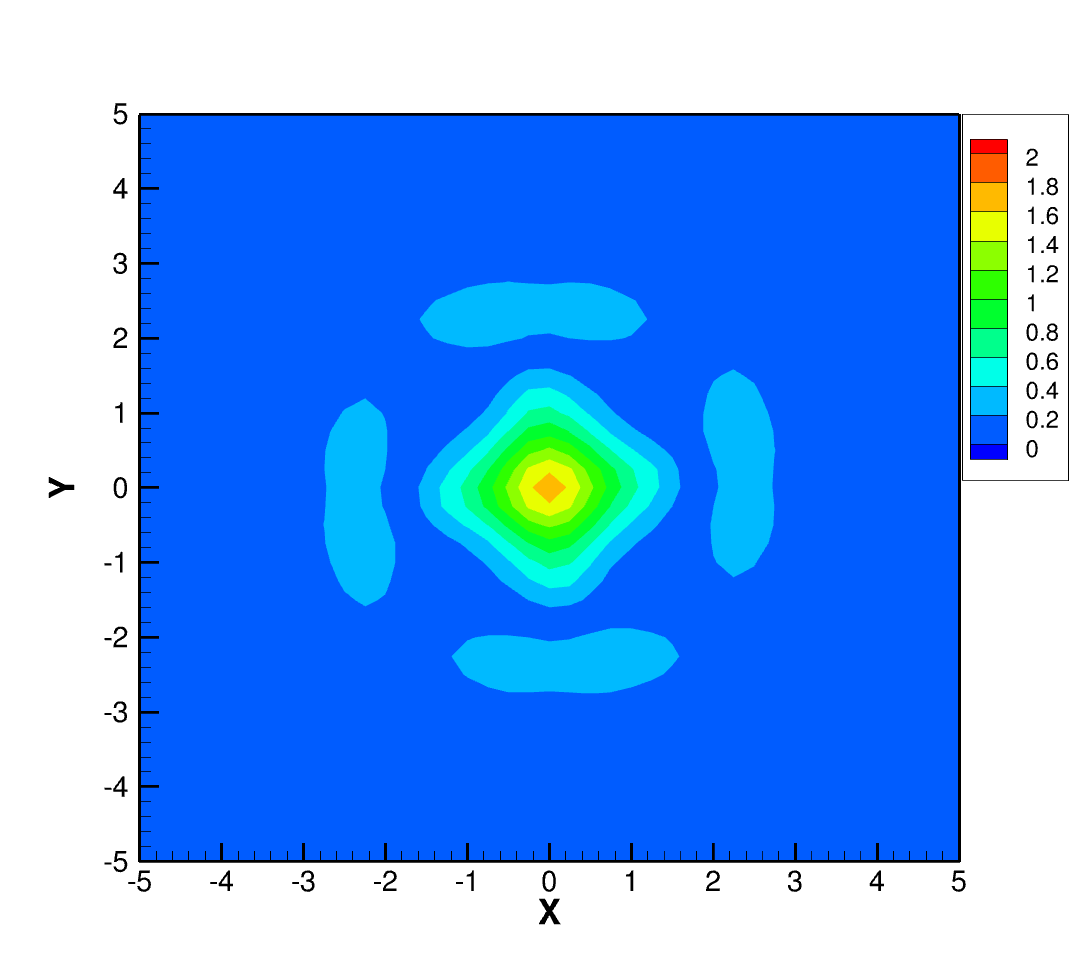
\includegraphics[clip=true, trim= 1.5cm 1.25cm 0.25cm 0.5cm,width=0.325\linewidth]{./figures/vortex3d/viscous/m2}}              
     \subfigure[EDDY at $z=2$]{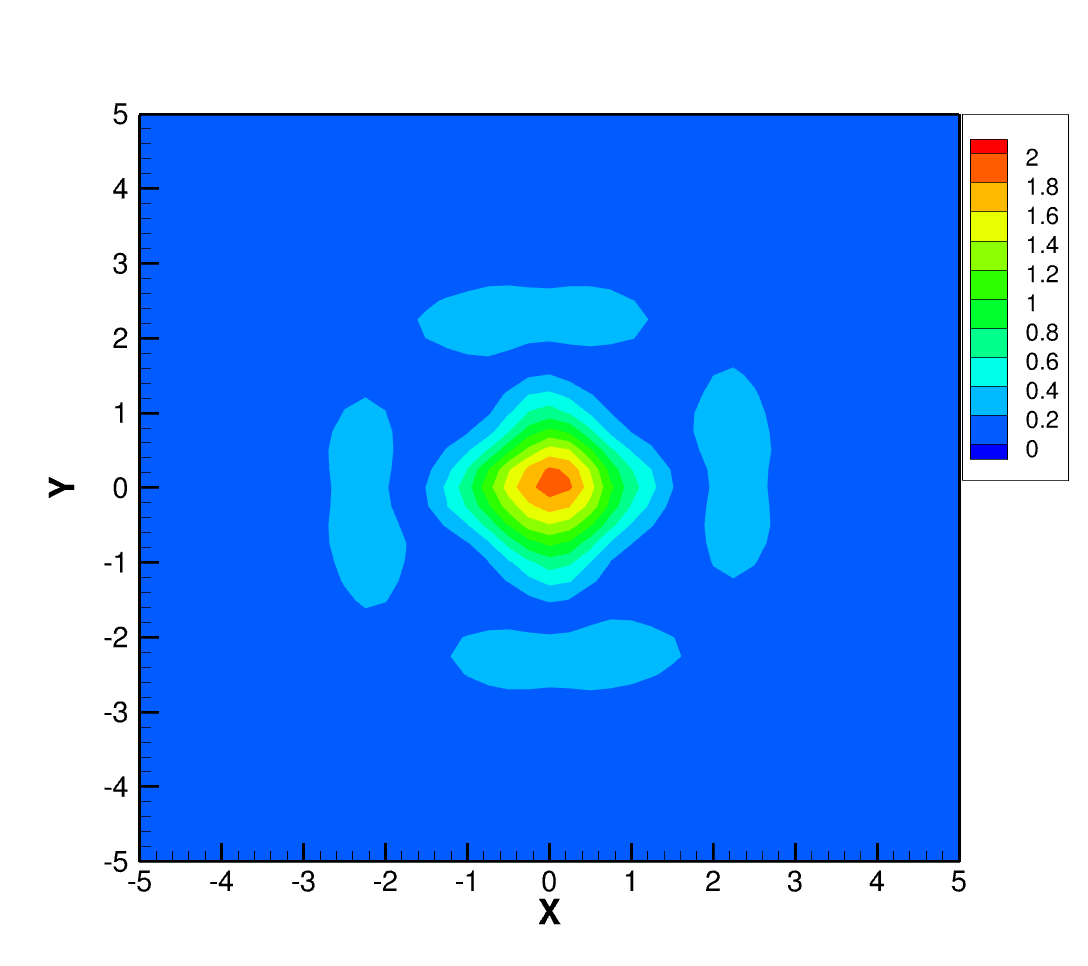
\includegraphics[clip=true, trim= 1.5cm 1.25cm 0.25cm 0.5cm,width=0.325\linewidth]{./figures/vortex3d/viscous/e2}}
     \subfigure[EDDY-P at $z=2$]{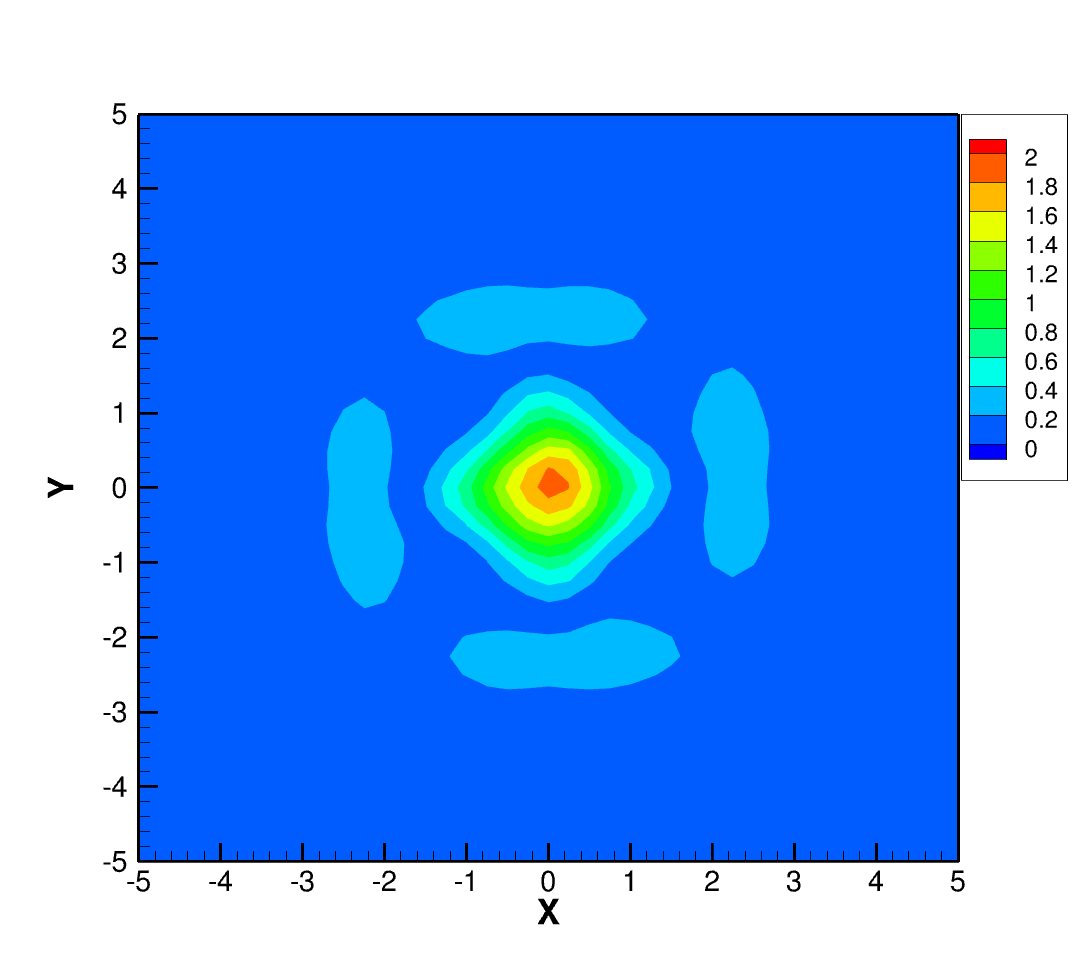
\includegraphics[clip=true, trim= 1.5cm 1.25cm 0.25cm 0.5cm,width=0.325\linewidth]{./figures/vortex3d/viscous/ep2}} 
     \subfigure[MUSCL at $z=3$]{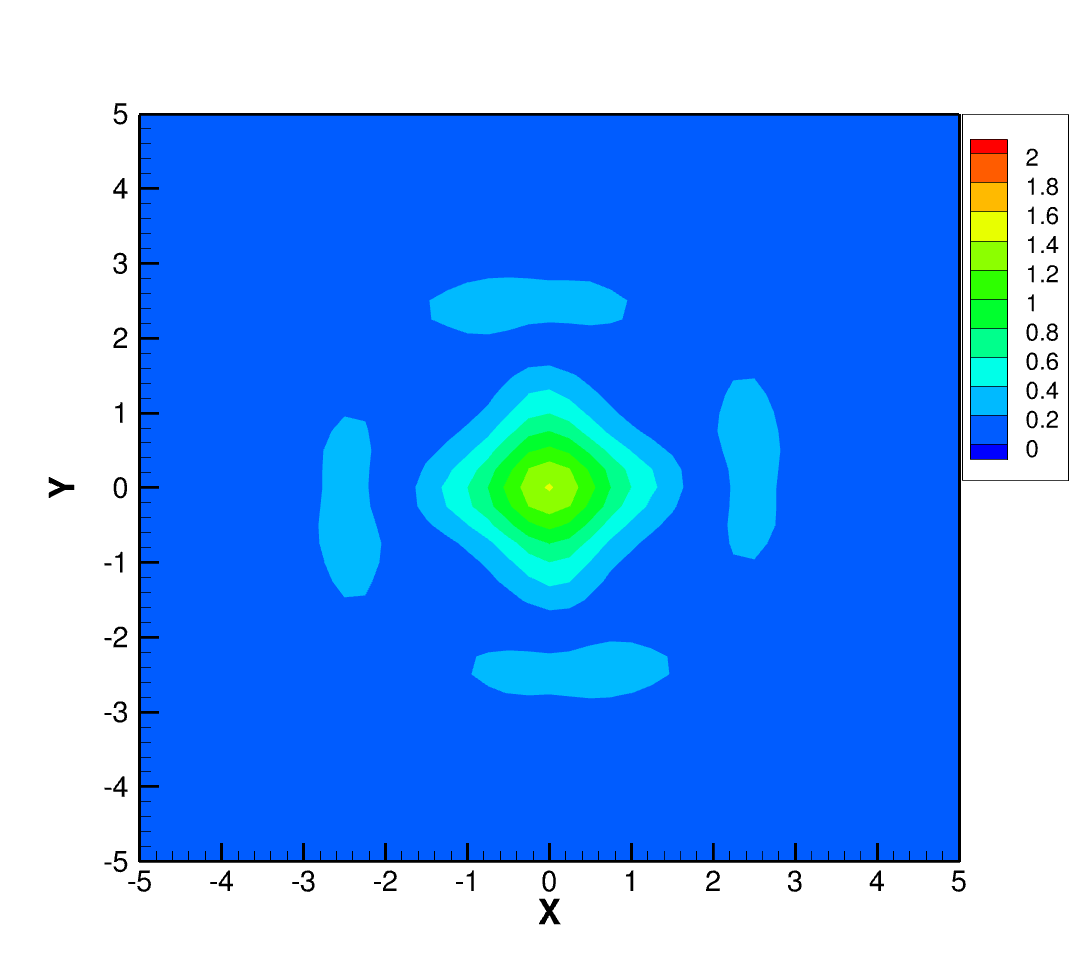
\includegraphics[clip=true, trim= 1.5cm 1.25cm 0.25cm 0.5cm,width=0.325\linewidth]{./figures/vortex3d/viscous/m3}}              
     \subfigure[EDDY at $z=3$]{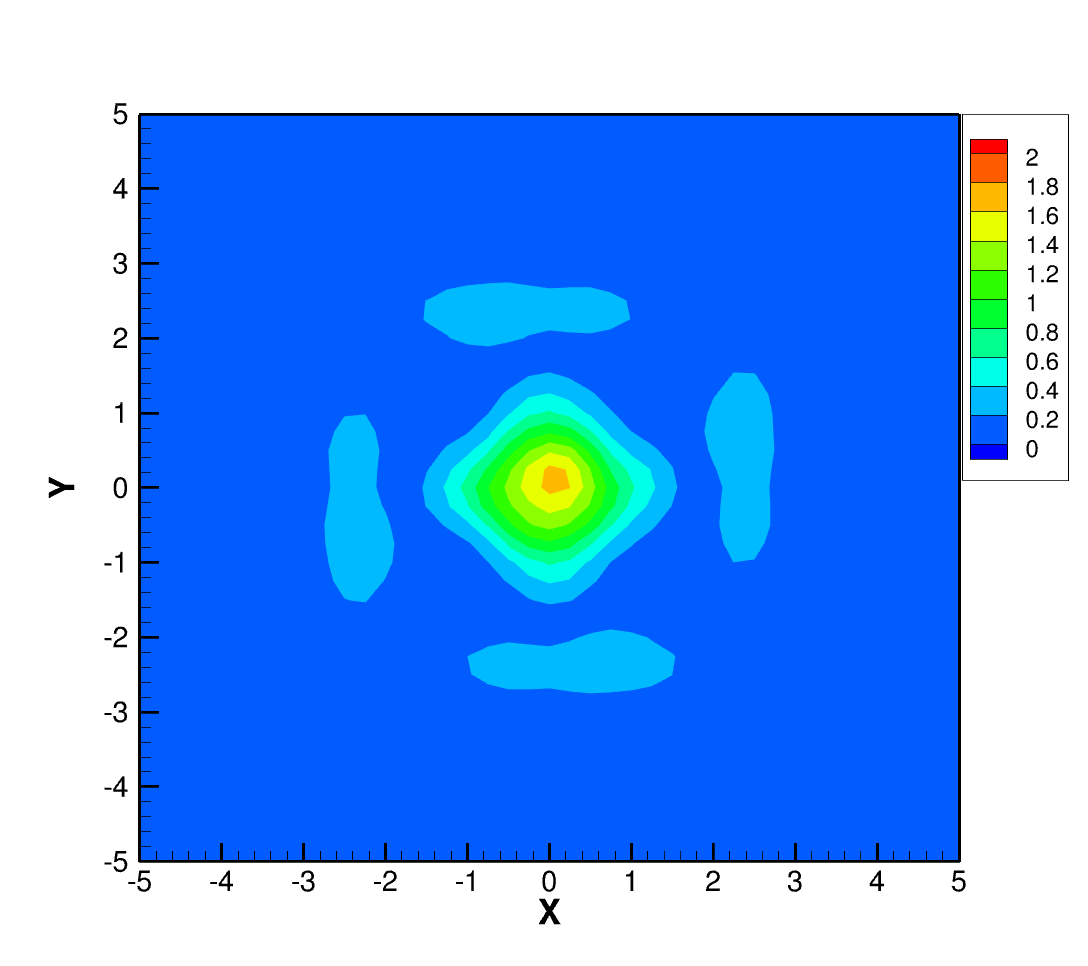
\includegraphics[clip=true, trim= 1.5cm 1.25cm 0.25cm 0.5cm,width=0.325\linewidth]{./figures/vortex3d/viscous/e3}}
     \subfigure[EDDY-P at $z=3$]{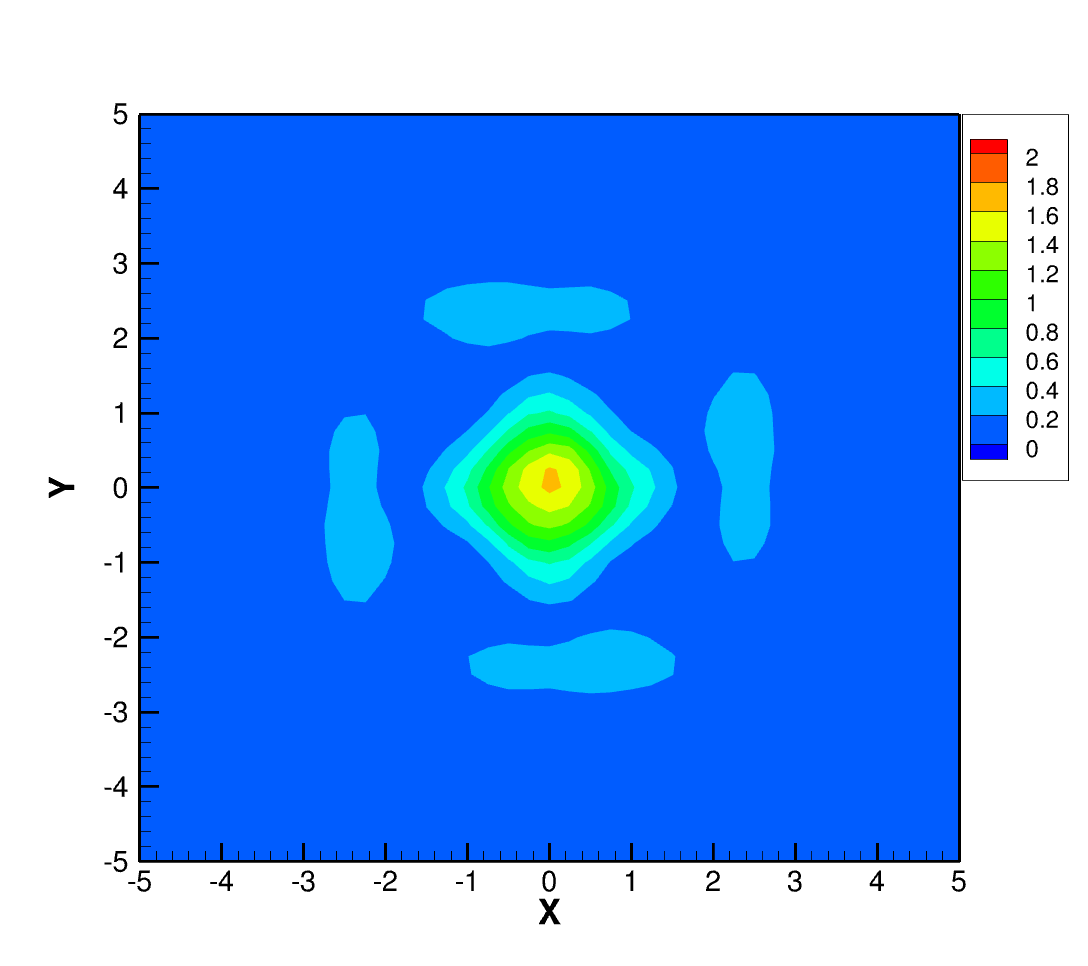
\includegraphics[clip=true, trim= 1.5cm 1.25cm 0.25cm 0.5cm,width=0.325\linewidth]{./figures/vortex3d/viscous/ep3}}                               
     \caption{Vorticity contours at different locations for three schemes.}
     \label{vortv}
\end{figure}
%%%%%%%%%%%%%%%%%%%%%%%%%%%%%%%%%%%%%%%%%%%%%%%%%%%%%%%%%%%%%%%%
%%%%%%%%%%%%%%%%%%%%%%%%%%%%%%%%%%%%%%%%%%%%%%%%%%%%%%%%%%%%%%%%
%%%%%%%%%%%%%%%%%%%%%%%%%%%%%%%%%%%%%%%%%%%%%%%%%%%%%%%%%%%%%%%%
%\begin{figure}[t]  
%\centering
%     \subfigure[]{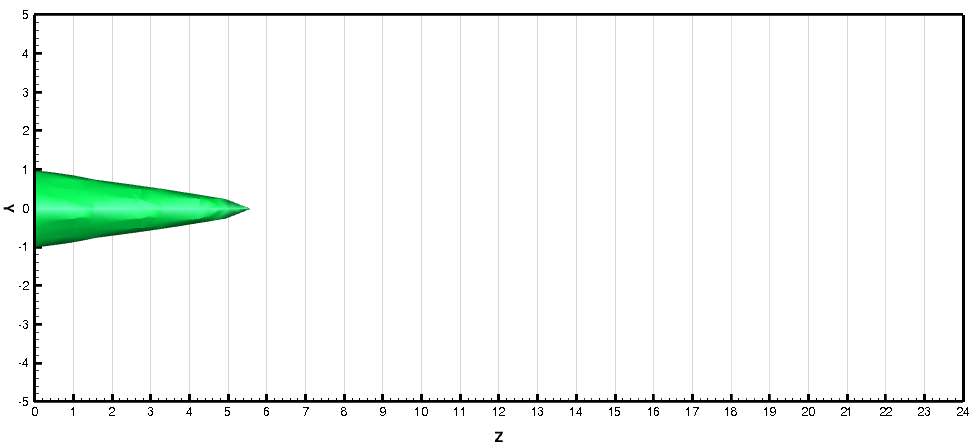
\includegraphics[clip=true, trim= 0.0cm 0.0cm 0.0cm 0.0cm,width=0.99\linewidth]{./figures/vortex3d/viscous/1}}               
%     \subfigure[]{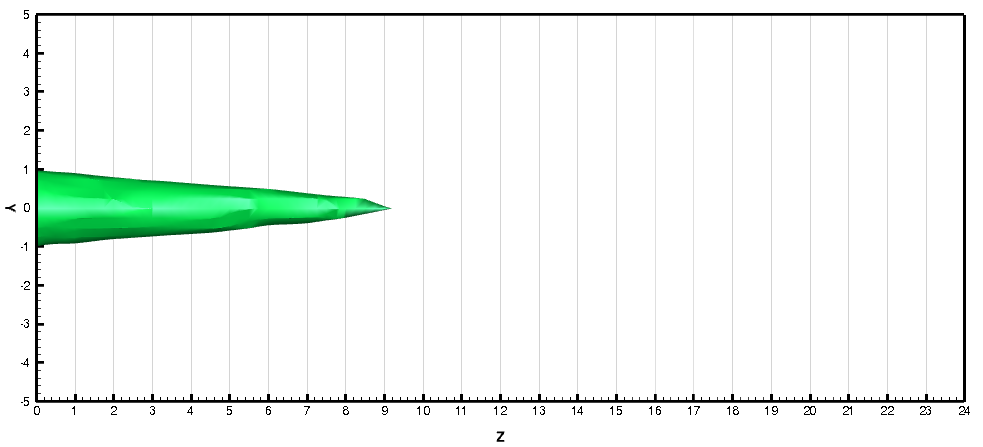
\includegraphics[clip=true, trim= 0.0cm 0.0cm 0.0cm 0.0cm,width=0.99\linewidth]{./figures/vortex3d/viscous/2}} 
%     \subfigure[]{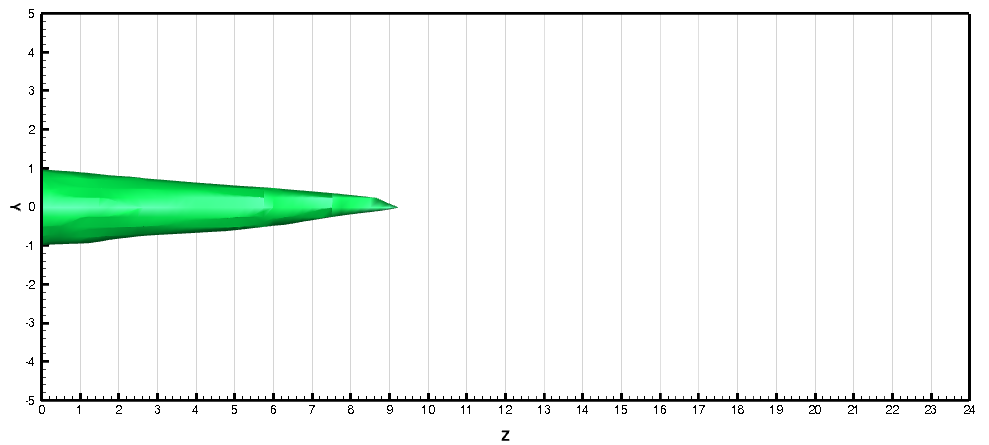
\includegraphics[clip=true, trim= 0.0cm 0.0cm 0.0cm 0.0cm,width=0.99\linewidth]{./figures/vortex3d/viscous/3}}               
%     \caption{Isosurface of vorticity magnitude computed by three schemes at $t=20$. (a)MUSCL (b)EDDY (c)EDDY-P.}
%     \label{iso}
%\end{figure}
%%%%%%%%%%%%%%%%%%%%%%%%%%%%%%%%%%%%%%%%%%%%%%%%%%%%%%%%%%%%%%%%
%%%%%%%%%%%%%%%%%%%%%%%%%%%%%%%%%%%%%%%%%%%%%%%%%%%%%%%%%%%%%%%%
%%%%%%%%%%%%%%%%%%%%%%%%%%%%%%%%%%%%%%%%%%%%%%%%%%%%%%%%%%%%%%%%
\begin{figure*}[t]  
\centering
     \subfigure[]{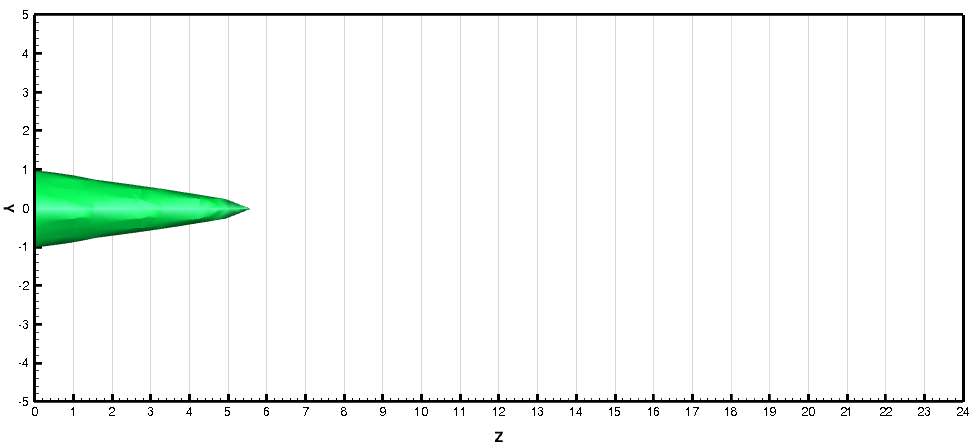
\includegraphics[clip=true, trim= 0.0cm 0.0cm 0.0cm 0.0cm,width=0.325\linewidth]{./figures/vortex3d/viscous/1}}               
     \subfigure[]{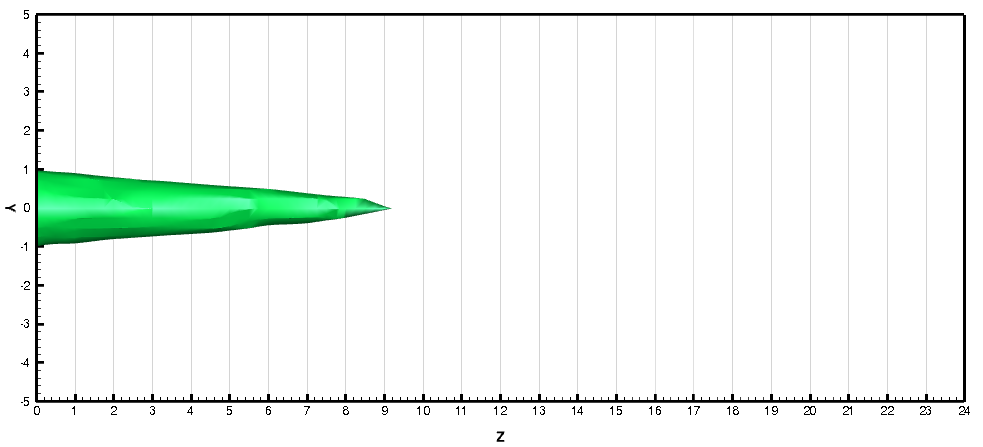
\includegraphics[clip=true, trim= 0.0cm 0.0cm 0.0cm 0.0cm,width=0.325\linewidth]{./figures/vortex3d/viscous/2}} 
     \subfigure[]{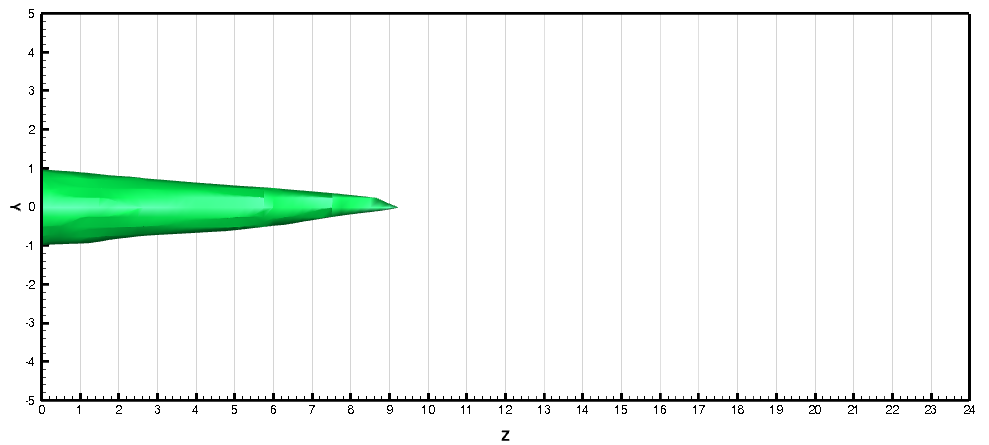
\includegraphics[clip=true, trim= 0.0cm 0.0cm 0.0cm 0.0cm,width=0.325\linewidth]{./figures/vortex3d/viscous/3}}               
     \caption{Isosurface of vorticity magnitude computed by three schemes at $t=20$. (a)MUSCL (b)EDDY (c)EDDY-P.}
     \label{iso}
\end{figure*}

